\section{Техническое задание}
\subsection{Основание для разработки}

Основанием для разработки является задание на курсовую работу «\Тема».

\subsection{Цель и назначение разработки}

Задачами данной разработки являются:
\begin{itemize}
\item осуществление загрузки аудиофайла и извлеения аудиоданных;
\item реализация отображения аудиоданных посредством аудиодорожки;
\item создание способов обработки аудиоданных;
\item осуществление сохранения изменений и запись аудиофайла.
\end{itemize}

\subsection{Требования пользователя к интерфейсу программы}

Программа должна включать в себя:
\begin{itemize}
    \item возможность выбора аудиофайла;
    \item визуализацию аудиофайла;
    \item набор инструментов для манипуляции аудиофайлом;
    \item возможность сохранения аудиофайла;
\end{itemize}

Композиция программы представлена на рисунке ~\ref{test_image:image}.

\begin{figure}[ht]
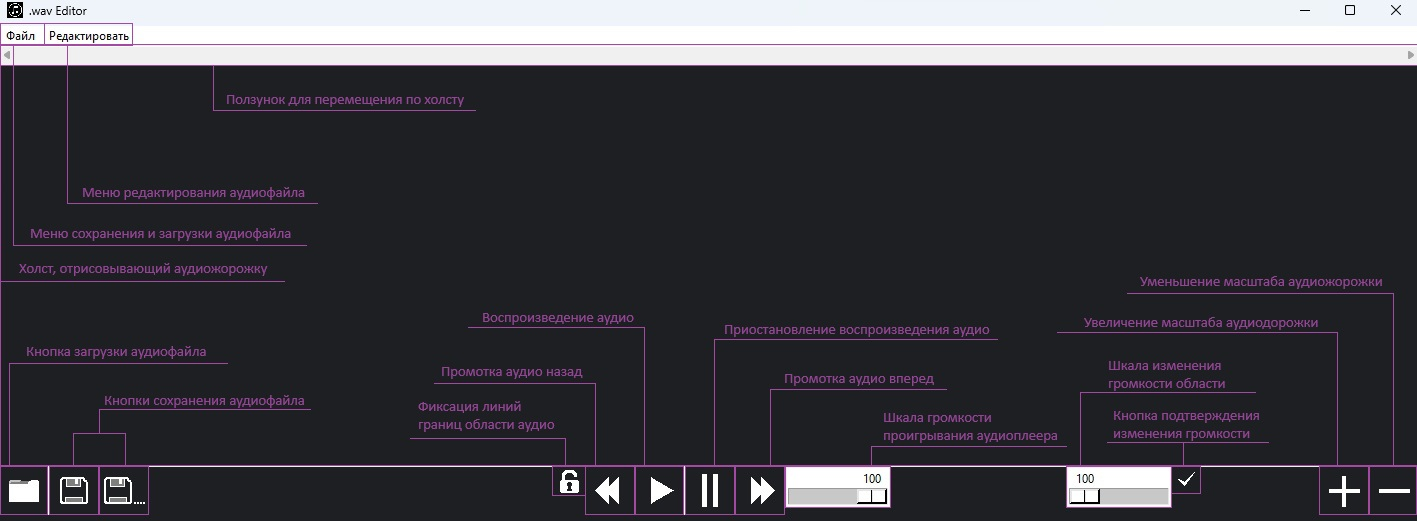
\includegraphics[width=1\linewidth]{test_image}
\caption{Композиция интерфейса программы}
\label{test_image:image}
\end{figure}
%\vspace{-\figureaboveskip} % двойной отступ не нужен (можно использовать, если раздел заканчивается картинкой)

\subsection{Моделирование вариантов использования}

Для разрабатываемой программы была реализована модель, которая обеспечивает наглядное представление вариантов использования аудиоредактора.

Она помогает в физической разработке и детальном анализе взаимосвязей объектов. При построении диаграммы вариантов использования применяется унифицированный язык визуального моделирования UML.

Диаграмма прецедентов (рис. \ref{diagram_choice:image}) описывает функциональное назначение разрабатываемой программы. То есть это то, что программа будет непосредственно делать в процессе своего функционирования. Проектируемая программа представляется в виде ряда прецедентов, предоставляемых системой актерам или сущностям, которые взаимодействуют с ней. Актером или действующим лицом является сущность, взаимодействующая с программой извне. Прецедент служит для описания набора действий, которые программа предоставляет актеру. 

На основании анализа предметной области в программе должны быть реализованы следующие прецеденты работы с аудиофайлом, все прецеденты осуществляются посредством взаимодействия с компонентами интерфейса:
\begin{enumerate}
\item Загрузка - возможность выбора аудиофайла для последующей визализации и редактирования.
\item Визуализация - отображение аудиоданных в виде аудиодорожки с возможностью увеличения и уменьшения масштаба, а также выбора необходимой области.
\item Прослушивание - возможность воспроизведения и остановки прослушивания аудио, также как и перемотки на определенное количество секунд вперед/назад.
\item Редактирование - наличие набора инструментов для редактирования аудиоданных, включающего в себя такие операции, как копирование, удаление, вставку, замену, обнуление, понижение громкости и добавление эффектов нарастания и затухания.
\item Сохранение - возможность записи измененных аудиоданных в WAV файл, как новый, так и оригинальный.
\end{enumerate}

\begin{figure}[ht]
	\includegraphics[width=1\linewidth]{diagram_choice}
	\caption{Диаграмма прецедентов}
	\label{diagram_choice:image}
\end{figure}

\subsubsection{Вариант использования "<Загрузка">}

Заинтересованные лица и их требования: пользователь желает загрузить аудиофайл для редактирования.

Предусловие: программа запущена, форматом аудиофайла является WAV.

Постусловие: аудио успешно загружено и подготовлено для последующего редактирования.

Основной успешный сценарий:
\begin{enumerate}
	\item Пользователь нажимает на кнопку загрузки.
	\item Программа открывает окно просмотра диска.
	\item Пользователь выбирает аудиофайл и подтверждает загрузку.
	\item Программа загружает аудиофайл и его данные в буфер.
\end{enumerate} 

\subsubsection{Вариант использования "<Увеличение/уменьшение масштаба">}

Заинтересованные лица и их требования: пользователю нужно более подробное визуальное представление аудиоданных.

Предусловие: программа запущена, загружен аудиофайл формата WAV, аудиодорожка успешно отрисована.

Постусловие: масштаб аудиодорожки изменен.

Основной успешный сценарий:
\begin{enumerate}
	\item Пользователь нажимает на кнопку увеличения/уменьшения масштаба.
	\item Программа перерисовывает аудиодорожку с большим/меньшим масштабом.
\end{enumerate} 

\subsubsection{Вариант использования "<Выбор области">}

Заинтересованные лица и их требования: пользователь хочет выбрать область для редактирования аудиоданных.

Предусловие: программа запущена, загружен аудиофайл формата WAV, аудиодорожка успешно отрисована.

Постусловие: установлена область редактирования.

Основной успешный сценарий:
\begin{enumerate}
	\item Пользователь нажимает ЛКМ и ПКМ для выбора границы начала и конца области соответственно.
	\item Программа устанавливает область редактирования в соответствие с запросами пользователя.
\end{enumerate} 

\subsubsection{Вариант использования "<Пуск">}

Заинтересованные лица и их требования: пользователь хочет воспроизвести аудио.

Предусловие: программа запущена, загружен аудиофайл формата WAV.

Постусловие: воспроизведение аудио.

Основной успешный сценарий:
\begin{enumerate}
	\item Пользователь нажимает на кнопку Пуск.
	\item Программа начинает воспроизведение аудио.
\end{enumerate} 

\subsubsection{Вариант использования "<Пауза">}

Заинтересованные лица и их требования: пользователь хочет остановить воспроизведение аудио.

Предусловие: программа запущена, загружен аудиофайл формата WAV, начато воспроизведение аудио.

Постусловие: остановка воспроизведения аудио.

Основной успешный сценарий:
\begin{enumerate}
	\item Пользователь нажимает на кнопку Пауза.
	\item Программа останавливает воспроизведение аудио.
\end{enumerate} 

\subsubsection{Вариант использования "<Пропустить">}

Заинтересованные лица и их требования: пользователь хочет пропустить несколько секунд аудио.

Предусловие: программа запущена, загружен аудиофайл формата WAV.

Постусловие: перемещение по аудиопотоку.

Основной успешный сценарий:
\begin{enumerate}
	\item Пользователь нажимает на кнопку перемотки аудио вперед/назад.
	\item Программа смещает момент начала воспроизведения аудио.
\end{enumerate} 

\subsubsection{Вариант использования "<Копирование">}

Заинтересованные лица и их требования: пользователь хочет скопировать выделенную область аудио.

Предусловие: программа запущена, загружен аудиофайл формата WAV, выбрана необходимая область.

Постусловие: копирование выбранной области.

Основной успешный сценарий:
\begin{enumerate}
	\item Пользователь открывает меню редактирования и выбирает вариант <"Копировать>".
	\item Программа успешно загружает выбранную область в буфер копирования.
\end{enumerate} 

\subsubsection{Вариант использования "<Вставить">}

Заинтересованные лица и их требования: пользователь хочет вставить скопированную оласть.

Предусловие: программа запущена, загружен аудиофайл формата WAV, скопирована желаемая и выбрана необходимая области.

Постусловие: вставка скопированной области.

Основной успешный сценарий:
\begin{enumerate}
	\item Пользователь открывает меню редактирования и выбирает вариант <"Вставить>".
	\item Программа успешно вставляет скопированную пользователем область.
\end{enumerate} 

\subsubsection{Вариант использования "<Заменить">}

Заинтересованные лица и их требования: пользователь хочет заменить выбранную область скопированной.

Предусловие: программа запущена, загружен аудиофайл формата WAV, скопирована желаемая и выбрана необходимая для замены области.

Постусловие: замена выбранной области скопированной.

Основной успешный сценарий:
\begin{enumerate}
	\item Пользователь открывает меню редактирования и выбирает вариант <"Заменить>".
	\item Программа успешно заменяет выбранную область на скопированную пользователем.
\end{enumerate} 

\subsubsection{Вариант использования "<Удаление">}

Заинтересованные лица и их требования: пользователь хочет пропустить несколько секунд аудио.

Предусловие: программа запущена, загружен аудиофайл формата WAV, выбрана необходимая область.

Постусловие: удаление выбранной области.

Основной успешный сценарий:
\begin{enumerate}
	\item Пользователь открывает меню редактирования и выбирает вариант <"Копировать>".
	\item Программа успешно загружает выбранную область в буфер копирования.
\end{enumerate} 

\subsubsection{Вариант использования "<Обнуление">}

Заинтересованные лица и их требования: пользователь хочет обнулить сигналы выбранной области.

Предусловие: программа запущена, загружен аудиофайл формата WAV, выбрана необходимая область.

Постусловие: обнуление сигналов выбранной области.

Основной успешный сценарий:
\begin{enumerate}
	\item Пользователь открывает меню редактирования и выбирает вариант <"Обнулить>".
	\item Программа успешно обнуляет сигналы выбранной области.
\end{enumerate} 

\subsubsection{Вариант использования "<Понижение громкости">}

Заинтересованные лица и их требования: пользователь хочет понизить громкость выбранной области.

Предусловие: программа запущена, загружен аудиофайл формата WAV, выбрана необходимая область и, на соответствующей шкале, желаемая громкость.

Постусловие: понижение громкости выбранной области.

Основной успешный сценарий:
\begin{enumerate}
	\item Пользователь нажимает на кнопку подтверждения или открывает меню редактирования и выбирает вариант <"Изменить громкость>".
	\item Программа успешно изменяет громкость выбранной области.
\end{enumerate} 

\subsubsection{Вариант использования "<Эффект нарастания/затухания">}

Заинтересованные лица и их требования: пользователь хочет добавить эффект нарастания/затухания для выбранной области.

Предусловие: программа запущена, загружен аудиофайл формата WAV, выбрана необходимая область.

Постусловие: добавление эффекта для области.

Основной успешный сценарий:
\begin{enumerate}
	\item Пользователь открывает меню редактирования и выбирает вариант <"Нарастание>" или <"Затухание>".
	\item Программа успешно применяет соответствующий эффект для выбранной области.
\end{enumerate} 

\subsubsection{Вариант использования "<Сохранение">}

Заинтересованные лица и их требования: пользователь хочет сохранить аудиоданные в аудиофайл.

Предусловие: программа запущена, загружен аудиофайл формата WAV.

Постусловие: сохранение аудиофайла.

Основной успешный сценарий:
\begin{enumerate}
	\item Пользователь загружает аудиофайл.
	\item Пользователь проводит все необходимые операции.
	\item Пользователь выбирает один из вариантов сохранения, нажав на соответствующую кнопку.
	\item Программа успешно записывает аудиоданные в файл формата WAV.
\end{enumerate} 

\subsection{Нефункциональные требования к программной системе}

\subsubsection{Требования к надежности}
В связи с тем, что работа в программе ведется не с самим файлом непосредственно, а с буфером данных, получаемых из него,
то даже при удалении исходного аудиофайла все данные о нем будут сохранены в случае, если они уже были загружены в программу.

\subsubsection{Требования к программному обеспечению}
Для реализации программы должен быть использован язык Python, а также связанные с ним библиотеки: Tkinter, PySDL, NumPy и Ctypes. Для корректной работы программы должен быть установлен Python версии не ниже 3.11.

\subsubsection{Требования к аппаратному обеспечению}
Для корректной работоспособности программы необходим процессор с 2 и более ядрами.
Объем оперативной памяти должен быть не менее 512 МБ.

\subsection{Требования к оформлению документации}

Разработка программной документации и программного изделия должна производиться согласно ГОСТ 19.102-77 и ГОСТ 34.601-90. Единая система программной документации.
